% Chapter Template

\chapter{Empirical Study} % Main chapter title

\label{Chapter4} % Change X to a consecutive number; for referencing this chapter elsewhere, use \ref{ChapterX}

%----------------------------------------------------------------------------------------
%	SECTION 1
%----------------------------------------------------------------------------------------
\section{Study Design}

As expected, para cumplir con el objetivo general de esta tesis se deben cumplir con los objetivos especificos, una vez estos sean completados a cabalidad entonces se tiene el objetivos general completado.

Explicar por qué se seleccionaron las herramientas (RIP, TestLab, etc)
Explicar las apps utilizadas en el estudio.

La idea es que estos objetivos especificos lleven o ayuden a llegar al cumplimiento de este objetivo general.

Se debe explicar cómo se cumplió con cada uno de ellos y al final explicar cómo se llegó a cumplir con el objetivo general

mostrar los resultados y analizarlos.

//TODO
two from the industry and two from the academic side. The first tool was Firebase Test Lab. it was selected for being widely used in industry and for also being a Google product. The second one, Monkey, was selected for being the most basic one and because it is also included in the SDK for developing Android Apps. The third one, Droidbot, was selected from the academic side. Droidbot has been a point of study for many researches. Many others tools have based their functionality on this tool. The last one is RIP, this tool was selected for being of special interest for us. It is our own exploration tool and is is currently an active project inside the Software Design Lab at University of Los Andes. 

Every tool was executed ten times per application, and every execution with a maximum time of 30 minutes. Some tools ended its exploration before the max time. 
The number of executions and the maximum time were arbitrary decisions that were made because of time limitations for the study. Although, during the study was notice that most of the tools ended the exploration or reached their maximum coverage within the first 15 minutes. Which means that the maximum time for exploration was more than enough in almost all cases. 
 



//TODO
Besides that, for this study, a set of 11 applications was used. This set is a subset of a set of open source applications utilised inside The Software Design Lab research group for other studies and tests, including RIP. Every APK in the subset should be successfully instrumented by InstruAPK, it should compile without any problem after instrumentation and it should be launch in an emulator without any issue after instrumentation.


\section{Context of the Study}


\begin{table}[t]
	\centering
	\caption{Applications used for the study}
	\label{tab:alufs}
	\resizebox{0.80\textwidth}{!}{
		\begin{tabular}{c c c c}
			App ID & Package Name & \# Methods Reported by APKAnalyzer & \# Methods Instrumented by InstruAPK\\
			\hline
			1 & appinventor.ai\_nels0n0s0ri0.MiRutina & 61993 & 9351\\
			2 & com.evancharlton.mileage & 4000 & 1162\\
			3 & com.fsck.k9 & 18799 & 7003\\
			4 & com.ichi2.anki & 32370 & 2209\\
			5 & com.workingagenda.devinettes & 19274 & 66 \\
			6 & de.vanitasvitae.enigmandroid & 13083 & 574 \\
			7 & info.guardianproject.ripple & 19429 & 100 \\
			8 & org.connectbot & 20606 & 1145\\
			9 & org.gnucash.android & 75473 & 504\\
			10 & org.libreoffice.impressremote & 14691 & 649\\
			11 & org.lumicall.android & 45784 & 540\\
			\hline
		\end{tabular}
	}
\end{table}

\begin{figure}[h]
\centering
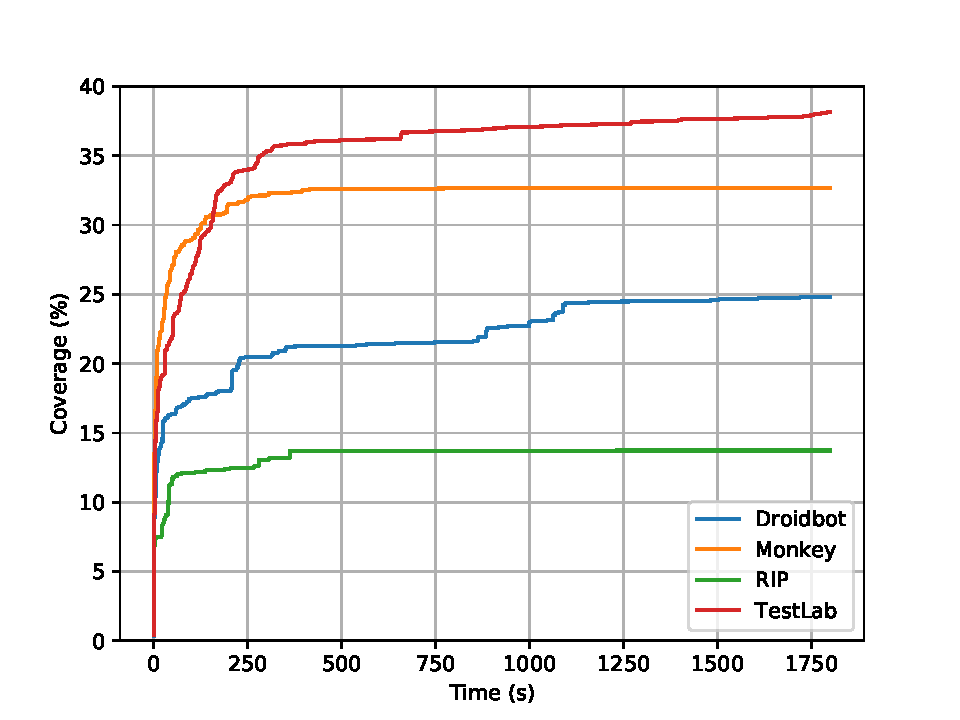
\includegraphics[width=0.8\textwidth]{../Figures/averageCoverageInstruAPK.pdf}
\caption{Average Method Coverage by Tool}\label{fig:averageCoverage}
\end{figure}

\begin{figure}[h]
\centering
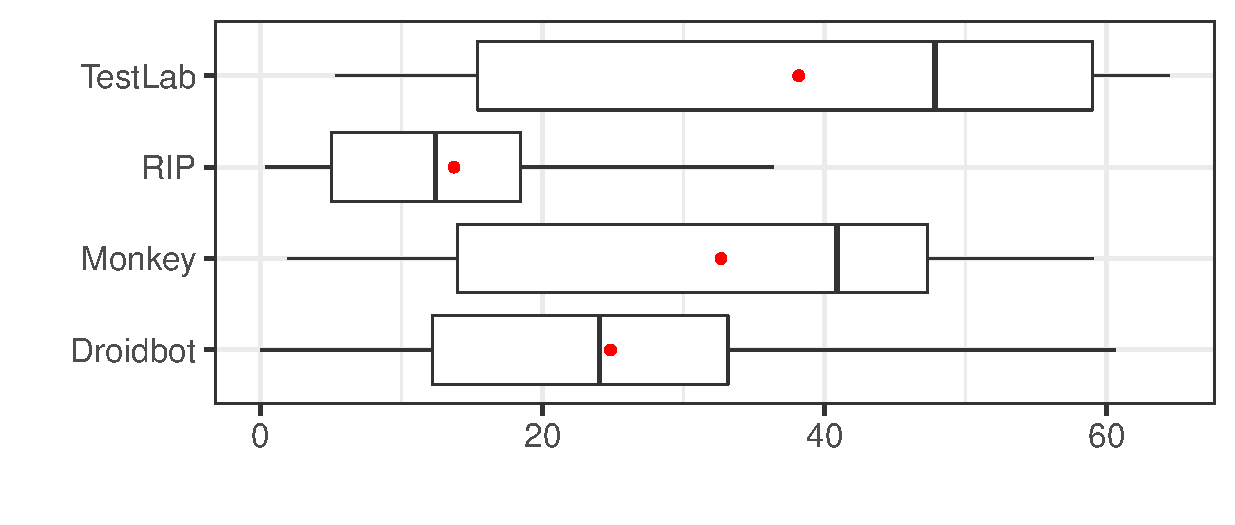
\includegraphics[width=0.8\textwidth]{../Figures/boxplotAccumulated.pdf}
\caption{Boxplot of Accumulated Coverage by Tool}\label{fig:boxplotAccumulated}
\end{figure}

\begin{figure}[h]
\centering
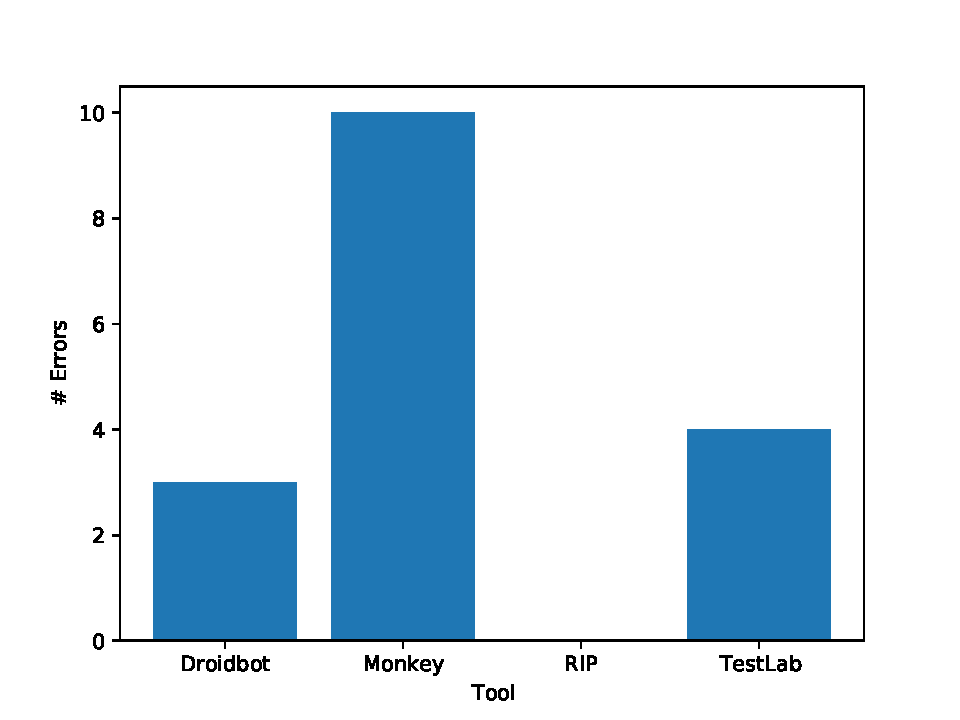
\includegraphics[width=0.8\textwidth]{../Figures/maxErrors.pdf}
\caption{Maximum Number of Errors Found by Tool}\label{fig:maxerrors}
\end{figure}

\begin{figure}[h]
\centering
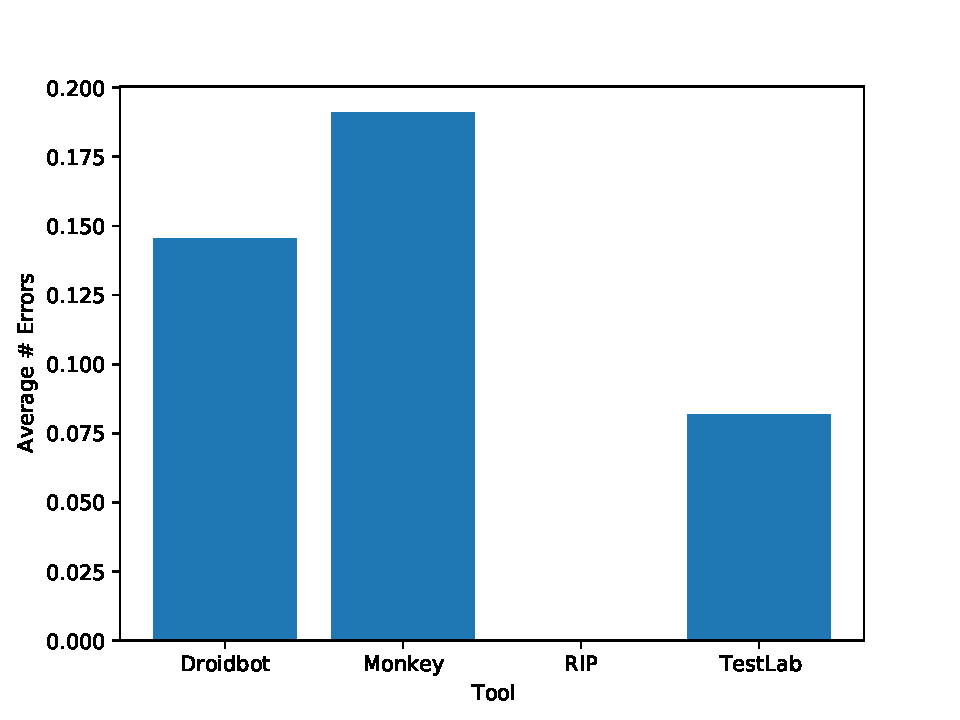
\includegraphics[width=0.8\textwidth]{../Figures/averageErrors.pdf}
\caption{Average Number of Errors Found by Tool}\label{fig:averagaerrors}
\end{figure}
